\chapter{Các công nghệ sử dụng}
\section{Xây dựng tính năng autoscaling với custom metrics (các thông số tùy chỉnh)}

\subsection{Định nghĩa}
\noindent Theo Google Cloud Platform\footnote{Dựa theo link: https://cloud.google.com/kubernetes-engine/docs/concepts/custom-and-external-metrics}, một \textit{custom metric} sẽ được truyền từ ứng dụng của bạn mà đang chạy trên Kubernetes.
\subsection{Đặt vấn đề}
\noindent Việc scale theo CPU và memory không hiệu quả với rest api.\\
\noindent Mặc dù các số liệu mặc định do Kubernetes cung cấp, chẳng hạn như mức sử dụng CPU và bộ nhớ dựa trên yêu cầu tài nguyên, rất hữu ích trong nhiều tình huống nhưng chúng có thể không đủ cho tất cả các ứng dụng. Mở rộng quy mô dựa trên giới hạn tài nguyên đảm bảo rằng ứng dụng của chúng ta có thể xử lý các khối lượng công việc khác nhau mà không đạt đến mức tài nguyên tối đa được phép. Số liệu tùy chỉnh cho phép chúng ta điều chỉnh hành vi mở rộng quy mô của HPA dựa trên nhu cầu cụ thể của ứng dụng, cho phép tự động điều chỉnh quy mô chính xác và hiệu quả hơn.
\subsection{Cơ sở lý thuyết}
\textit{Nội dung tiểu mục được tham khảo từ chung một nguồn}\footnote{https://learnk8s.io/autoscaling-apps-kubernetes}\\[0.5cm]
% \noindent Nói về việc prometheus dùng để thu thập và cung cấp api server cho external metrics. KEDA cung cấp ScaledObject, được build dựa trên HPA để phục vụ cho việc scale dựa trên các metric thu thập từ prometheus.\\
% \noindent Có thể để các tóm tắt bài viết vào đây.
Khi xác định tài nguyên cho Horizontal Pod Autoscaler, chúng ta cần phải xác định metric mà ta cần theo dõi.

% Nhưng làm cách nào Bộ chia tỷ lệ tự động của Horizontal Pod biết cách lấy được các số liệu này?

Horizontal Pod Autoscaler truy vấn các metrics này từ Metrics Registry.
\begin{figure}[H]
  \begin{center}
    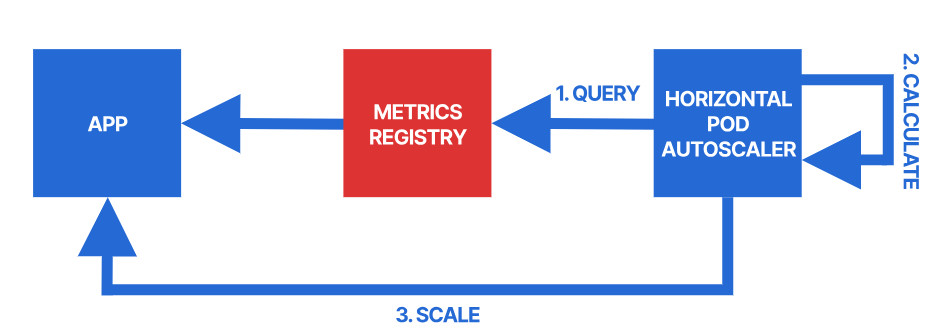
\includegraphics[scale=0.65]{images/phat/metrics_registry.jpg}
    \caption{Horizontal Pod Autoscaler queries flow}
  \end{center}
\end{figure}
Metrics Registry là vị trí trung tâm trong cluster nơi các metrics (dưới bất kỳ hình thức nào) được hiển thị cho clients (Horizontal Pod Autoscaler là một trong những ứng dụng clients này).

Mục đích Metrics Registry là cung cấp giao diện chuẩn cho client truy vấn các metrics.

Interface của Metrics Registry bao gồm 03 API riêng biệt:
\begin{itemize}
    \item The Resource Metrics API
    \item The Custom Metrics API
    \item The External Metrics API
\end{itemize}
\begin{figure}[H]
  \begin{center}
    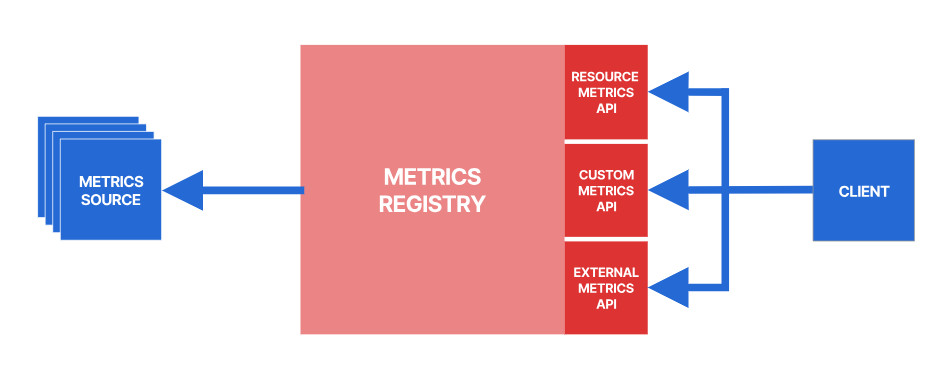
\includegraphics[scale=0.75]{images/phat/metrics_registry_API.jpg}
    \caption{Metrics Registry Interfaces}
  \end{center}
\end{figure}
Các API này được thiết kế để phục vụ các loại metrics khác nhau:
\begin{itemize}
    \item Resource Metrics API: số liệu sử dụng tài nguyên được xác định trước (CPU và bộ nhớ) của Pod và Node.
    \item Custom Metrics API: số liệu tùy chỉnh được liên kết với đối tượng nằm bên trong Kubernetes cluster.
    \item External Metrics API: số liệu tùy chỉnh được liên kết với đối tượng nằm bên ngoài Kubernetes cluster.
\end{itemize}
Vì vậy, để autoscale cho một ứng dụng, nhiệm vụ của chúng ta không chỉ là xác định cấu hình Horizontal Pod Autoscaler mà cũng phải hiển thị metrics mong muốn của mình thông qua Metric Registry.\\[0.5cm]
Đối với mỗi Metric API, chúng ta cần có Metric API Server tương ứng và chúng ta cần định cấu hình cho nó để hiển thị một metric cụ thể thông qua Metric API.\\[0.5cm]
Hơn nữa, chúng ta cần một Metrics Collector để thu thập các metrics mong muốn từ các nguồn (ví dụ: từ Pod của ứng dụng) và cung cấp chúng cho Metric API Server.
\begin{figure}[H]
  \begin{center}
    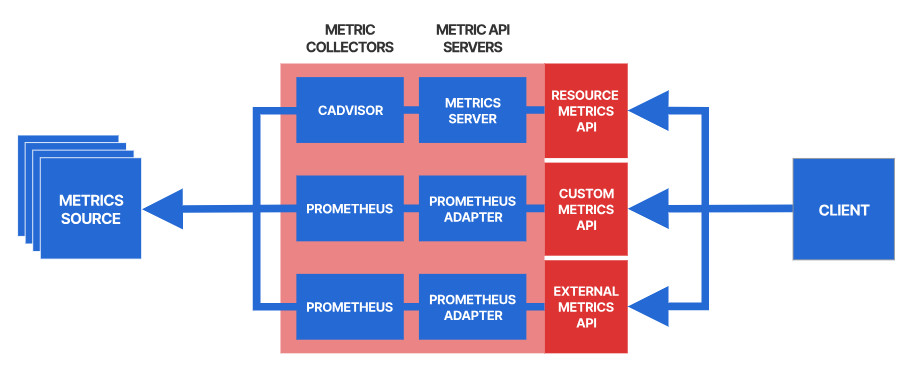
\includegraphics[scale=0.80]{images/phat/metric_registry_detail.jpg}
    \caption{Metrics Registry components}
  \end{center}
\end{figure}
Vì vậy, để expose metric thông qua một trong các API Metrics, chúng ta phải thực hiện các bước sau:
\begin{itemize}
    \item Cài đặt Metrics Collector (ví dụ: Prometheus) và định cấu hình nó để thu thập metric mong muốn (ví dụ: từ Pod của ứng dụng của bạn).
    \item Cài đặt Metric API Server (ví dụ: Prometheus Adapter) và định cấu hình nó để hiển thị từ Metrics collector thông qua Metrics API tương ứng.
\end{itemize}
$\ast$ \textbf{KEDA} sẽ hoạt động với vai trò như một Metric API Server, dùng để biên dịch các metric nhận được từ external server về các dạng dữ liệu mà HPA có thể hiểu được để tiến hành scale thông qua HPA. Như vậy khi sử dụng KEDA thì chúng ta sẽ không cần phải sử dụng Metrics Server từ K8s. Với KEDA chúng ta có 1 khái niệm là \textit{ScaledObject}, khi tạo ScaleObject nó là một phiên bản mở rộng của HPA để thực hiện việc scale pod.
\subsection{Các công nghệ được sử dụng}
\subsubsection{Prometheus}
% TODO: Các phần này cần tự tìm thêm các nguồn khác để tìm hiểu
\textbf{a. Định nghĩa \footnote{https://www.tigera.io/learn/guides/prometheus-monitoring/prometheus-kubernetes}}\\[0.5cm]
Prometheus là một dịch vụ theo dõi và cảnh báo về hệ thống. Prometheus rất thích hợp với những hệ thống Microservices và có các dịch vụ Listening. Một hệ thống theo dõi chủ động như Prometheus sẽ giúp người quản trị phát hiện sớm những dấu hiệu cảnh báo xấu.\\[0.5cm]
Đối với những công việc liên quan đến Queue Job, mối nguy cơ luồng xử lý bị loop hoặc stop rất lớn. Lý do có thể đến từ tài nguyên phần cứng hoặc phần mềm được cài đặt không chính xác. Khi đó việc xem log của dịch vụ đó rất khó hoặc phụ thuộc vào may mắn. Với Prometheus các thông tin luôn được cập nhật và khi xảy ra lỗi, chúng ta vẫn có thể xem lại dữ liệu theo dõi một cách dễ dàng qua API của Prometheus.\\[0.5cm]
\textbf{b. Kiến trúc Prometheus \footnote{https://www.devopsschool.com/blog/what-is-prometheus-and-how-it-works}}

\begin{figure}[H]
  \begin{center}
    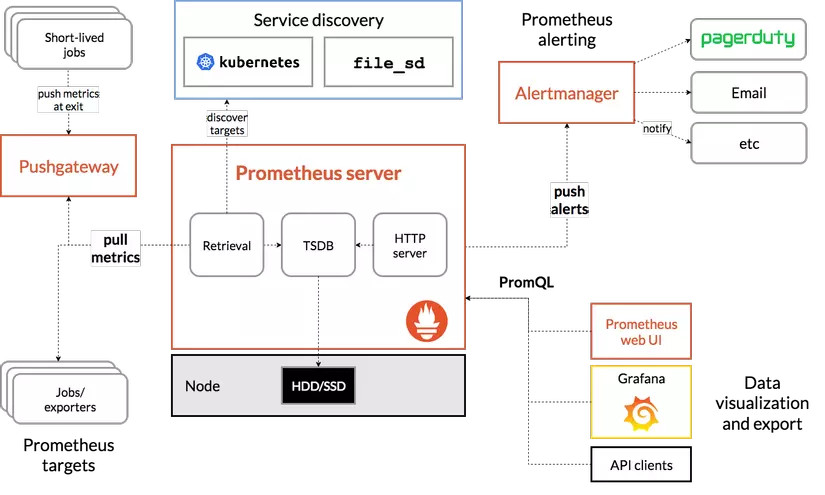
\includegraphics[scale=0.45]{images/phat/prometheus_architecture.jpg}
    \caption{Kiến trúc Prometheus}
  \end{center}
\end{figure}
\textbf{Các thành phần của hệ thống}\\[0.5cm]
\indent Có thể chia kiến trúc Prometheus thành 03 thành phần chính sau: 
\begin{enumerate}
    \item Prometheus Server
    \item Alert Manager
    \item Grafana
\end{enumerate}
\indent Cụ thể các thành phần chi tiết như sau:
\begin{itemize}
    \item \textbf{Prometheus Server}: thành phần chính thu thập, xử lý và lưu trữ dữ liệu chuỗi thời gian (time-series data).
    Nó chủ động liên tục lấy dữ liệu từ các điểm cuối (endpoints) của các dịch vụ và ứng dụng để thu thập thông tin về các metrics.
    Dữ liệu thu thập được được lưu trữ tại máy chủ Prometheus.
    \item \textbf{Push Gateway Prometheus}: sử dụng để hỗ trợ các job có thời gian thực hiện ngắn (tạm thời). Đơn giản là các tác vụ công việc này không tồn tại đủ lâu để Prometheus chủ động lấy dữ liệu. Vì vậy mà các dữ liệu chỉ số (metrics) sẽ được đẩy về Push Gateway rồi đẩy về Prometheus Server.
    \item \textbf{Jobs/Exporters}: hỗ trợ giám sát các dịch vụ hệ thống và gửi về Prometheus theo chuẩn Prometheus mong muốn.
    \item \textbf{AlertManager}: dịch vụ quản lý, xử lý các cảnh báo (alert).
    \item \textbf{TSDB \textit{(cơ sở dữ liệu chuỗi thời gian)}}: Prometheus sử dụng TSDB để lưu trữ tất cả dữ liệu một cách hiệu quả. Theo mặc định, tất cả dữ liệu được lưu trữ cục bộ. Tuy nhiên, để tránh single point of failure, có các tùy chọn tích hợp bộ lưu trữ từ xa cho Prometheus TSDB.
\end{itemize}
\textbf{c. Prometheus WorkFlow \footnote{https://prometheus.io/docs/introduction/overview/\#architecture}}
\begin{itemize}
    \item \textbf{Thu Thập Metric}
    \begin{itemize}
        \item Prometheus chủ động liên tục lấy dữ liệu từ các mục tiêu bằng cách gửi các yêu cầu HTTP đến các điểm cuối của chúng (thường là /metrics).
        \item Dữ liệu thu thập được được lưu trữ tại máy chủ Prometheus.
    \end{itemize}
    \item \textbf{Lưu trữ dữ liệu}
    \begin{itemize}
        \item Prometheus lưu trữ dữ liệu chuỗi thời gian tại máy chủ. Định dạng lưu trữ được tối ưu hóa để truy vấn và thống kê nhanh chóng.
    \end{itemize}
    \item \textbf{Truy vấn và ngôn ngữ biểu diễn (PromQL):}
    \begin{itemize}
        \item Prometheus cung cấp một ngôn ngữ truy vấn mạnh mẽ (PromQL) cho việc truy vấn và tổng hợp dữ liệu chuỗi thời gian.
        \item Toán tử, hàm và bộ lựa chọn cho phép người dùng biểu diễn các truy vấn phức tạp và tạo bảng điều khiển tùy chỉnh.
    \end{itemize}
    \item \textbf{Cảnh báo}
    \begin{itemize}
        \item Prometheus có thể định nghĩa các quy tắc cảnh báo dựa trên biểu diễn PromQL. Khi một quy tắc cảnh báo được kích hoạt, một cảnh báo được gửi đến AlertManager.
        \item AlertManager sau đó xử lý và chuyển tiếp cảnh báo dựa trên các tuyến đường và ứng dụng thông báo đã được cấu hình.
    \end{itemize}
    \item \textbf{Trực quan hóa}
    \begin{itemize}
        \item Grafana (một plugin của Prometheus) thường được sử dụng như một công cụ trực quan để tạo bảng điều khiển cho các metrics của Prometheus. Grafana hỗ trợ Prometheus như một nguồn trực quan hóa dữ liệu bằng biểu đồ và bảng biểu.
    \end{itemize}
\end{itemize}
\subsubsection{KEDA}
% TODO: Các phần này cần tự tìm thêm các nguồn khác để tìm hiểu
\textbf{a. Định nghĩa \footnote{https://KEDA.sh/docs/2.12/concepts/}}\\[0.5cm]
KEDA \textit{(Kubernetes-Based Event-Driven Autoscaler)} là một Kubernetes-based Event Driven Autoscaler. Với KEDA, chúng ta có thể điều chỉnh quy mô của bất kỳ container nào trong Kubernetes dựa trên số lượng sự kiện (event) cần được xử lý.\\[0.5cm]
KEDA là một thành phần nhẹ và đơn mục đích có thể được thêm vào bất kỳ Kubernetes cluster nào. KEDA hoạt động cùng với các thành phần Kubernetes tiêu chuẩn như Horizontal Pod Autoscaler và có thể mở rộng chức năng mà không cần ghi đè hoặc sao chép. Với KEDA, bạn có thể ánh xạ rõ ràng các ứng dụng bạn muốn sử dụng quy mô theo sự kiện, trong khi các ứng dụng khác vẫn tiếp tục hoạt động. Điều này làm cho KEDA trở thành một lựa chọn linh hoạt và an toàn để chạy cùng với bất kỳ ứng dụng hoặc Kubernetes framework nào khác.\\[0.5cm]
\textbf{b. Kiến trúc \footnote{https://devtron.ai/blog/introduction-to-kubernetes-event-driven-autoscaling-KEDA/}}
 
\begin{figure}[H]
  \begin{center}
    \includegraphics[scale=0.32]{images/phat/KEDA Architecture.jpg}
    \caption{Kiến trúc KEDA}
  \end{center}
\end{figure}

\textbf{Các thành phần chính}
\begin{itemize}
    \item \textbf{Event sources}\\
    Đây là các nguồn kích hoạt/sự kiện bên ngoài mà KEDA sử dụng để thay đổi số lượng nhóm. Prometheus, RabbitMQ và Apache Pulsar là một số ví dụ về nguồn sự kiện.
    \item \textbf{Scalers}\\
    Các nguồn sự kiện được giám sát bằng cách sử dụng công cụ chia tỷ lệ, công cụ này tìm nạp số liệu và kích hoạt quy mô Deployments hoặc Jobs dựa trên các sự kiện.
    \item \textbf{Metrics adapter}\\
    Metrics adapter lấy số liệu từ bộ chia tỷ lệ và chuyển đổi hoặc điều chỉnh chúng thành dạng mà thành phần HPA/bộ điều khiển có thể hiểu được.
    \item \textbf{Controller}\\
    Controller hoạt động dựa trên các số liệu do bộ điều hợp cung cấp và mang lại trạng thái triển khai mong muốn được chỉ định trong ScaledObject.
\end{itemize}
\textbf{c. Cách thức hoạt động}\\[0.5cm]
KEDA hoạt động bằng cách tương tác với Kubernetes API và sử dụng các adapters để kết nối và theo dõi các nguồn sự kiện bên ngoài hệ thống Kubernetes. Dưới đây là một mô tả tổng quan về cách KEDA hoạt động:
\begin{itemize}
    \item \textbf{Triển Khai KEDA}
    \begin{itemize}
        \item KEDA được triển khai trên cụm Kubernetes như một Operator hoặc thông qua các tài nguyên Kubernetes tiêu chuẩn.
    \end{itemize}
    \item \textbf{Sự Kiện và adapter}
    \begin{itemize}
        \item KEDA sử dụng các adapters để theo dõi các nguồn sự kiện bên ngoài hệ thống Kubernetes. Các adapters này có thể là các thành phần được tích hợp sẵn để xử lý các loại sự kiện cụ thể.
        \item Ví dụ: Nếu bạn muốn mở rộng dựa trên kích thước hàng đợi RabbitMQ, bạn có thể sử dụng adapter RabbitMQ của KEDA.
    \end{itemize}
    \item \textbf{Tích Hợp với Pod Scaler}
    \begin{itemize}
        \item Pod Scaler là một thành phần quan trọng của KEDA và chịu trách nhiệm về việc mở rộng (hoặc giảm) số lượng pods dựa trên sự kiện được theo dõi.
        \item Khi có sự kiện xảy ra, Pod Scaler sẽ quyết định xem cần mở rộng, giảm số lượng pods, hoặc duy trì tình trạng hiện tại.
    \end{itemize}
    \item \textbf{Kết Nối với Kubernetes API}
    \begin{itemize}
        \item Pod Scaler tương tác với Kubernetes API để điều chỉnh số lượng pods. Nó có thể thay đổi các ReplicaSets hoặc Deployments để tăng giảm quy mô.
    \end{itemize}
    \item \textbf{Chia Sẻ Thông Tin với Metrics Server}
    \begin{itemize}
        \item Pod Scaler thông tin về trạng thái hiện tại và các quyết định của mình với Metrics Server. Metrics Server cung cấp thông tin về hiệu suất và trạng thái của các pods.
    \end{itemize}
    \item \textbf{Môi Trường Linh Hoạt và Quản Lý Tài Nguyên}
    \begin{itemize}
        \item KEDA cung cấp một môi trường linh hoạt cho việc xử lý sự kiện và quản lý tài nguyên. Nó có thể mở rộng dựa trên nhiều loại sự kiện và chia sẻ nguồn lực giữa nhiều ứng dụng.
    \end{itemize}
\end{itemize}
Tóm lại, KEDA hoạt động như một thành phần giám sát và quản lý tài nguyên mạnh mẽ trong môi trường Kubernetes. Nó tương tác với các nguồn sự kiện bên ngoài và tự động điều chỉnh số lượng pods của ứng dụng để đảm bảo rằng tài nguyên được triển khai hiệu quả và hiệu suất tốt nhất.
\subsubsection{K6}
% TODO: Các phần này cần tự tìm thêm các nguồn khác để tìm hiểu
\textbf{a. Bài toán đặt ra \footnote{https://techmaster.vn/posts/36882/performance-testing-voi-k6}}\\[0.5cm]
Giả sử chúng ta code 1 API mà khi dùng postman tạo request thì thấy cũng có response. Tuy nhiên, sau khi đưa vào sử dụng thì ngày nào cũng thấy bị log lỗi do request gửi vào liên tục, dẫn đến tình trạng cao tải, thành ra tính năng thì có, nhưng gần như không dùng được, vì vậy để giúp xác định tắc nghẽn trong một hệ thống, thiết lập một đường cơ sở để kiểm thử trong tương lai, hỗ trợ điều chỉnh hiệu suất hiệu quả, xác định sự phù hợp mục tiêu và yêu cầu hiệu suất, và thu thập dữ liệu hoạt động liên quan khác để giúp các bên liên quan đưa ra quyết định liên quan đến chất lượng chung của các ứng dụng đang được kiểm thử thì việc dùng performance testing là một lựa chọn tối ưu.\\[0.5cm]
Performance Testing là một loại kiểm thử nhằm xác định mức độ đáp ứng, băng thông, độ tin cậy và/hoặc khả năng mở rộng của hệ thống dưới một khối lượng làm việc/truy cập nhất định.\\[0.5cm]
Hiện tại có rất nhiều công cụ hỗ trợ kiểm thử hiệu năng như Jmeter, Grinder, LoadComplete, K6, v.v.\\[0.5cm]
\textbf{b. Định nghĩa \footnote{https://anhdevhamhoc.com/view/16-k6-inovative-and-effective-performace-testing-tool}}\\[0.5cm]
K6 là một công cụ mã nguồn mở được đặc biệt thiết kế để thực hiện kiểm tra hiệu suất và khả năng chịu tải các ứng dụng web và API. Do Load Impact phát triển, K6 nhằm mục tiêu đơn giản hóa quá trình kiểm tra hiệu năng và cung cấp kết quả đáng tin cậy, giúp các nhà phát triển và quản trị hệ thống đưa ra các quyết định thông minh về hiệu suất của ứng dụng.\\[0.5cm]
\textbf{c. Ưu điểm của K6}
\begin{itemize}
    \item \textbf{Sử dụng JavaScript làm ngôn ngữ lập trình}\\
    K6 được xây dựng bằng JavaScript, một ngôn ngữ lập trình phổ biến và dễ tiếp cận. Điều này giảm thiểu thời gian học và cho phép các nhà phát triển sử dụng kiến thức JavaScript hiện có để tạo ra các kịch bản kiểm tra hiệu suất một cách hiệu quả.
    \item \textbf{Dễ cài đặt và sử dụng}\\
    K6 có cấu trúc đơn giản và rõ ràng, giúp người dùng nhanh chóng cài đặt và bắt đầu tạo các bài kiểm tra. Chỉnh sửa và xem xét mã cũng trở nên dễ dàng, tiết kiệm thời gian và tăng hiệu suất công việc.
     \item \textbf{Kiểm tra tải đơn giản}\\
     K6 hỗ trợ kiểm tra tải tập trung (stress testing), kiểm tra tải phân tán (load testing), và kiểm tra hiệu suất chức năng (functional testing). Điều này giúp người dùng có cái nhìn tổng quan về hiệu năng ứng dụng trong nhiều tình huống khác nhau.
     \item \textbf{Hỗ trợ đa nền tảng}\\
     K6 chạy trên nhiều nền tảng, bao gồm Windows, macOS và Linux. Điều này cho phép người dùng thực hiện các bài kiểm tra từ các môi trường khác nhau một cách dễ dàng.
     \item \textbf{Tích hợp linh hoạt và thư viện mở rộng}\\
     K6 hỗ trợ nhiều thư viện mở rộng bổ sung, giúp người dùng mở rộng khả năng kiểm tra của mình. Nó cũng tích hợp tốt với các công cụ phổ biến như Grafana và InfluxDB để hiển thị kết quả kiểm tra hiệu suất một cách trực quan.
     \item \textbf{Hiệu suất mạnh mẽ}\\
     K6 được thiết kế để xử lý số lượng lớn yêu cầu đồng thời và đáp ứng trong thời gian thực. Điều này giúp các chuyên gia hiệu suất thực hiện kiểm tra trong các điều kiện khắc nghiệt mà vẫn duy trì độ chính xác cao.
\end{itemize}